The resampling algorithm takes $N$ samples with coordinates $\bm{x}$ and
generates local polynomial fits at $M$ resampling points with coordinates
$\bm{v}$.
In this case, the ``local'' region for a single resampling point $m$ is defined
by a K-dimensional ellipsoid centered on $\bm{v}_m$.
The principle axes of the ellipsoid are given as a user supplied parameter
$\omega$ so that equation of the ellipsoid centered on point $m$ is given as

\begin{equation}
    \sum_{k=1}^{K}{\frac{(x_k - v_{m, k})^2}{\omega_k^2}} = 1
    \label{eq:equation11}
\end{equation}

The window region of point $m$ contains the set of samples $\Omega_m$ where sample
$i$ is included when

\begin{equation}
    i \in \Omega_m ~ \vert ~
        \sum_{k=1}^{K}{\frac{(x_{i, k} - v_{m, k})^2}{\omega_k^2}} \leq 1
    \label{eq:equation12}
\end{equation}

This window region will be constant for all resampling points.
Therefore, it should be chosen carefully as it defines the subset of samples
that are to be considered ``local'' for the LPR of each resampling point.
Although there is no strict limit to the size of the window in each dimension,
it should be chosen so that there are sufficient samples to perform a
polynomial fit of the desired order in most cases (see
section~\ref{subsubsec:order-rejection}).
Since $\omega$ is constant, determining $\omega$ for measurements consisting of
variable sample densities can be difficult.
It may be necessary to set $\omega$ to a large value in order to ensure fits occur
at certain resampling points.

If the instrumental response of the observing device is of importance, then
the window size should be chosen to represent a maximum distance for any
coupling effects.
For example, FIFI-LS reductions use a default window of
$3 \times \text{fwhm}_{\bar{\lambda}}$ in the spatial dimensions.
If distance weighting is enabled (see section~\ref{subsec:weighting}), and
$\sigma_x \ll \omega$, there is no significant consequence for the final result
with increased $\omega$.
Computationally, however, the window size increases the number of operations by
$\mathcal{O}(\omega^{K})$ assuming uniform sampling density, and should be
given extra consideration in higher dimensional reductions.
Figure~\ref{fig:resampling_window} gives a graphical representation of the
window in 3 dimensions.

\subsection{Search Problem}\label{subsec:search-problem}

In many cases, both $M$ and $N$ are large, and deriving $\Omega$ for all $M$
resampling points is computationally expensive.
To shorten processing time, the reduction is performed in parallel with each
thread performing a search on set of samples that are guaranteed to be close to
another set of resampling points.
This is accomplished by dividing up the sample coordinate space into regularly
spaced K-orthotopes (blocks) with the width in dimension $k$ equal to
$\omega_k$.
Binning resampling points and samples into blocks is a quick and easy procedure.
For any given block, the search for samples within the window region of any
resampling point in that block should be limited to the block itself, and all
immediately neighboring blocks as shown in figure~\ref{fig:block_neighbors}.

\begin{figure}[H]
  \begin{center}
  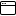
\includegraphics[width=0.5\linewidth]{images/window.png}
  \caption{The window region centered around point $\bm{v}_m$ in 3-dimensions.
           All samples falling within the shaded region will be included in
           the fit.  The principle axes ($\omega$) of the ellipsoid defining
           the bounds of the window are supplied by the user.}
  \label{fig:resampling_window}
  \end{center}
\end{figure}

\begin{figure}[H]
  \begin{center}
  \includegraphics[width=0.5\linewidth]{images/block_neighbors.png}
  \caption{Division of a 2-D sample space into blocks.  The search for
           samples inside the window region of all resampling points within
           the target block is limited to immediately neighboring blocks.}
  \label{fig:block_neighbors}
  \end{center}
\end{figure}

The procedure used to bin samples and points into blocks simply by assigning an
integer index to any given coordinate $\bm{x}$ in K-dimensions using

\begin{equation}
    \text{block}_{i, k} = \left\lfloor
        \frac{x_{i,k} - min(\bm{x_k})}{\omega_k}
    \right\rfloor
    \label{eq:equation13}
\end{equation}

for coordinate $i$ in dimension $k$ where $\lfloor\cdots\rfloor$ indicates the
floored value.
All neighboring blocks (the ``neighborhood'') including the block itself may
then be found by simply applying the kernel

\begin{equation}
    \text{neighborhood}_{i, k} = \text{block}_{i, k} + [-1, 0, 1]
    \label{eq:equation14}
\end{equation}

Once the block indices for all samples and points have been found, reductions
are performed in parallel over all blocks.
Each thread in the parallel reduction is sent a block of resampling points
along with its neighborhood of samples as shown in
figure~\ref{fig:parallel_reduction}.
Every resampling point in a thread is then processed in serial, first
determining which samples in the neighborhood are inside the window region
$\Omega_m$ of point $m$, and then deriving a fitted value at that location
(figure~\ref{fig:single_thread_reduction}).

\begin{figure}[H]
  \begin{center}
  \includegraphics[width=0.8\linewidth]{images/parallel.png}
  \caption{Left: Samples (blue dots) and resampling points (red crosses)
           divided into blocks for parallel reduction.  Right: Four threads
           of the parallel reduction, each containing a single block of
           resampling points (red grid squares) and its surrounding
           neighborhood of samples (blue grid squares).}
  \label{fig:parallel_reduction}
  \end{center}
\end{figure}

\begin{figure}[H]
  \begin{center}
  \includegraphics[width=\linewidth]{images/single_thread_reduction.png}
  \caption{Left: A single thread of the parallel reduction containing a set
           of resampling points (crosses) and samples (blue dots).  Each
           resampling point will be processed in series.  Right: All samples
           within the window region ($\Omega_m$) of point $m$ at coordinate
           $v_m$ will be included in the fit.}
  \label{fig:single_thread_reduction}
  \end{center}
\end{figure}

\subsection{Distribution Checks}\label{subsec:distribution-checks}

Before deriving a fit from the samples in the window region $\Omega_m$ of
about coordinate $v_m$ of resampling point $m$, a number of checks may be
performed.
These ensure that a polynomial fit of the desired order is possible, and the
position of the resampling point relative to the sample distribution will
result in a representative fit.

\subsubsection{Edge Rejection}\label{subsubsec:edge-rejection}

Polynomial fits (especially higher order polynomials) generally become
increasingly less representative of the samples from which they were derived
away from the center of the sample distribution.
A simple one-dimensional example shown in figure~\ref{fig:distribution_error_1d}
illustrates this deviation.

Away from the center of the distribution ($\bar{x} = 0$), both the deviation
and error on the fit begin to increase significantly, and it would be
undesirable to attempt a fit in such regions.
Therefore, the user may supply an ``edge threshold'' parameter
($\beta_{edge} > 0$) effectively defining an ``edge'' around the center of the
distribution.
No fitting will be permitted for any resampling point located outside of this
edge, and the value of the fit for any rejected point will be set to a
user-defined failure value.

\begin{figure}[H]
  \begin{center}
  \includegraphics[width=\linewidth]{images/distribution_error_1d.png}
  \caption{A $3^{rd}$ order polynomial fit (red) to the samples (blue).  The
           shaded red area is the $1\sigma$ error on the fit.}
  \label{fig:distribution_error_1d}
  \end{center}
\end{figure}

For a single dimension, we define the edge threshold parameter such that

\begin{equation}
    f(x)=\begin{cases}
        \hat{c}_m \cdot \Phi(v_m), & \textrm{if }
             | v_m - \bar{x} | \leq \sigma_x / \beta_{edge} \\
         \textrm{Failure value}, & \textrm{otherwise.}
    \end{cases}
    \label{eq:equation15}
\end{equation}

As $\beta_{edge}$ increases, the acceptable fitting region becomes more
concentrated about the center of the distribution ($\bar{\bm{x}}$).
In multiple dimensions, the covariance of the sample distribution
($\bm{\Sigma_x}$) is used, allowing the additional benefit of preventing fits
away from colinear type distributions.
For $K > 1$, the following exclusion is applied:

\begin{equation}
    f(x)=\begin{cases}
        \hat{c}_m \cdot \Phi(v_m), & \textrm{if }
             \sqrt{(\bm{v}_{m} - \bar{\bm{x}})^{T}
             {\Sigma_x}^{-1}(\bm{v}_m - \bar{\bm{x}})}
             \leq \beta_{edge}^{-1}\\
         \textrm{Failure value}, & \textrm{otherwise.}
    \end{cases}
    \label{eq:equation16}
\end{equation}

The point rejection region for a 2-dimensional sample distribution is
illustrated in figure~\ref{fig:distribution_error_2d} using an edge threshold
parameter $\beta_{edge}$ = 0.5, rejecting any fits occurring at more than
$2\sigma_x$ from the center of the sample distribution.

\begin{figure}[H]
  \begin{center}
  \includegraphics[width=0.75\linewidth]{images/distribution_error_2d.png}
  \caption{Edge rejection with $\beta_{edge}=0.5$.  No fits will be attempted
           more than $2\sigma_x$ from the center of the sample distribution
           (blue dots).  The fit exclusion area is shaded red and lines of
           constant $\sigma_x$ (Mahalanobis distance) are plotted as red dashed
           lines.}
  \label{fig:distribution_error_2d}
  \end{center}
\end{figure}

\subsubsection{Polynomial Order Rejection}
\label{subsubsec:order-rejection}

For the terms of a polynomial equation to be linearly independent over each
dimension, we require that there be at least $n_{order}$ samples to fit for
a given order $\bm{o}$, where

\begin{equation}
    n_{order} = \prod_{k=1}^{K}{(o_k + 1)}
    \label{eq:equation17}
\end{equation}

For example, two samples can uniquely define a first order (linear)
1-dimensional polynomial so long as those samples occupy unique coordinates.
However, those same two points can be modelled exactly by an infinite number of
higher order polynomials.
There is currently one mandatory and two optional polynomial order checks.
In all cases it is mandatory that

\begin{equation}
    | \Omega_m | \geq n_{order}
    \label{eq:equation18}
\end{equation}

where $| \Omega_m |$ indicates the cardinality (size, or number of samples) of
the set $\Omega_m$ for point $m$.
If the above condition is not met, the fit is aborted, and a failure value is
returned for the value at $v_m$.
In general, we want a ``best fit'' solution (in a least-squares sense) where
$| \Omega_m | > n_{order}$.
However, equation~\ref{eq:equation18} only requires that an exact fit is
possible.
If the user can guarantee that the samples are uniformly distributed, then
the procedure may be stopped here to save processing time.

The second step checks the number of unique coordinates in each dimension $k$
such that

\begin{equation}
    | \{ x_{i, k} \forall i \in \Omega_m \} | > o_k
    \label{eq:equation19}
\end{equation}

where $|\{\cdots\}|$ gives the cardinality (number of unique values) of the
sample coordinates for a given dimension.
The above check ensures that we have enough unique terms to allow for matrix
inversion in equations~\ref{eq:equation9} and~\ref{eq:equation10}.
Depending on how the user has defined $\beta_{edge}$
(see~\ref{subsubsec:edge-rejection}), this may allow for extrapolation at any
point within the window.

The final check ensures that there are enough samples to provide for a
least-squares best fit solution, and that any fitting occurs within the bounds
defined by the samples.
For a fit to occur,

\begin{align}
    |\{x_{i, k} \forall i \in \Omega_m \, \vert x_{i, k} < v_{m, k}\}| \geq o_k
    \nonumber \\
    |\{x_{i, k} \forall i \in \Omega_m \, \vert x_{i, k} > v_{m, k}\}| \geq o_k
    \label{eq:equation:20}
\end{align}

ensuring that $|\Omega_m| \geq 2 n_{order}$.

Examples of these three order checking algorithms are shown in
figure~\ref{fig:order_check}.
If the sample distribution does not meet the criteria defined in the order
checking algorithm, the returned fit value will be set to a user defined
failure value.

\begin{figure}[H]
  \begin{center}
  \includegraphics[width=\linewidth]{images/order_check.png}
  \caption{The three available edge checking algorithms shown in order of
           increasing robustness from left to right.  Samples (black dots)
           are regularly spaced at $\Omega / 2$ in the horizontal direction,
           and $\Omega / 6$ in the vertical direction.  Regions in which
           fits may occur are shaded green.}
  \label{fig:order_check}
  \end{center}
\end{figure}


\subsection{Weighting}\label{subsec:weighting}

Weighted polynomial regression is a method by which some samples in the local
polynomial fit have a stronger influence on the solution of the best fit
coefficients, as defined in equation~\ref{eq:equation10}.
Weighting may be based on the measurement error associated with each sample,
the position of a sample relative to each resampling point, or a combination of
both error and position.

The weighting applied to point $m$ is given as

\begin{equation}
    diag(W_m) = w_{\sigma, i} w_{\delta}(x_{i, m})\, \vert \, i \in \Omega_m
    \label{eq:equation21}
\end{equation}

where $\Omega_m$ is the local subset of samples included in the fit for point
$m$.
If positional (distance) weighting is not applied, then $w_\delta = 1$, and
error weighting is disabled when $w_\sigma=1$.
If no weighting occurs, then $W = I$, where $I$ is an identity matrix of rank
$|\Omega_m|$, and the notation $|.|$ indicates the cardinality (size or number
of unique values) in the set.

\subsubsection{Error Weighting}\label{subsubsec:error-weighting}

If the $1\sigma$ measurement error of sample $i$ is known ($\sigma_{y_i}$), the
associated weighting factor is:

\begin{equation}
    w_{\sigma, i} = \frac{1}{\sigma_{y_i}^2}
    \label{eq:equation23}
\end{equation}

The following figure (\ref{fig:error-weighting}) shows an example of fitting
with and without error weighting.

\begin{figure}[H]
  \begin{center}
  \includegraphics[width=0.75\linewidth]{images/error_weighting.png}
  \caption{An example of the application of error weighting in 1-dimension.
           Two of the samples shown with large error bars will skew the
           fit away from the underlying function if errors are not accounted
           for.}
  \label{fig:error-weighting}
  \end{center}
\end{figure}

\subsubsection{Distance Weighting}
\label{subsubsec:distance-weighting}

Distance weighting applies higher significance to samples that are closer to
the resampling point.
For the solution to converge effectively, the weighting kernel should be a
non-negative, bounded probability function (\citet{Gu15}).
Two popular functions are the Epanechnikov and Gaussian kernels, of which we
have opted for the Gaussian function as it has some desirable qualities that
are exploited during the adaptive weighting formulation (see
section~\ref{subsec:adaptive-weighting}).
The distance weighting applied to a single sample $i$ at coordinate $x_i$ for
a local polynomial fit centered on resampling point $m$ at coordinate $v_m$ is
given as

\begin{equation}
        w_{(\delta, i, m)} =
            exp \left(
                   -\sum_{k=1}^{K}{\frac{(v_{m, k} - x_{i, k})^2}{\alpha_k}}
                \right)
        \label{eq:equation25}
\end{equation}

where $\alpha$ is a user supplied smoothing parameter which may vary for each
dimension ($k$).
As $\alpha \rightarrow 0$, closer samples gain increasing influence over the
fit, whereas larger $\alpha$ values result in more equal weighting between
samples, irrespective of distance.
Note that in terms of the bandwidth given in equation~\ref{eq:equation70},
$h = \sqrt{\alpha}$.
We also frequently use the equation defining a multivariate Gaussian where

\begin{equation}
    w_{\delta} = exp \left(-(v - x)^T A^{-1} (v - x) \right)
    \label{eq:equation77}
\end{equation}

where $A = diag(2 \sigma_w^2) = diag(\alpha)$, and $\sigma_w$ is the standard
deviation of the Gaussian.
An example of distance weighting, and the effect of modifying $\alpha$ can be
seen in figure~\ref{fig:standard-distance-weighting}.

\begin{figure}[H]
  \begin{center}
  \includegraphics[width=0.75\linewidth]{images/standard_distance_weighting.png}
  \caption{The effect of distance weighting on a second order polynomial fit to
           samples generated using $y=\cos(\pi x)$.  The smoothing parameter
           ($\alpha$) can be modified to increase the influence of samples in
           the fit based on distance from the resampling point ($\Delta x$).}
  \label{fig:standard-distance-weighting}
  \end{center}
\end{figure}

\subsection{Adaptive Weighting}\label{subsec:adaptive-weighting}

If the data we wish to model can be easily represented by a smooth function,
then standard distance weighting may produce an acceptable fit.
However, when the underlying function contains a mix of structures of
varying complexity, a single distance weighting parameter may not be adequate.
This is alleviated somewhat by allowing the bandwidth parameter $h$ in
equation~\ref{eq:equation70} to vary at each resampling point, and is
extensively discussed by~\citet{Fan96b} and~\citet{Masry1996} amongst others.

Most methods seek to find the optimal smoothing parameter by minimizing
the mean squared error given in equation~\ref{eq:equation20}, balancing
the leading bias and variance.
In the case where we have supplied measurement errors, this does not always
result in what one may consider an ``optimal fit''.
This is especially true in the case of FIFI-LS where minimizing the overall
MSE results in highly spurious fits.
An alternative presented here, defines the optimal fit as one in which the
reduced chi-squared statistic ($\chi_r^2$), given in
equation~\ref{eq:equation75}, is equal to one.
When the measurement error is known, $\chi_r^2 > 1$ indicates a poor fit which
does not adequately represent the data.
Conversely, a fit where $\chi_r^2 < 1$ is over-fitting the data, and can be
thought of as fitting to the noise.
Therefore, our goal in determining an optimal smoothing parameter is to get
$\chi_r^2 \to 1$, rather than minimizing the MSE, which could likely result
in $\chi_r^2 \ll 1$.

We accomplish this by performing an initial test reduction using both distance
and error weighting where

\begin{equation}
    W = W_{\delta} W_{\sigma} = diag(w_{\delta, i} w_{\sigma, i}) =
        diag(\frac{w_{\delta, i}}{\sigma_{y, i}^2})
    \label{eq:equation27}
\end{equation}

and propagate the theoretical and stochastic variance as defined in
equations~\ref{eq:equation24} and~\ref{eq:equation76}.
We assume that the two measurements are related by

\begin{equation}
    \chi_r^2 = \frac{\text{Var} \{f(\bm{v}\, |\, \hat{c}_v) \}}
                    {\text{Var} \{f(\bm{v}\, |\, r)\}}
    \label{eq:equation26}
\end{equation}

Now, for a set of $n$ error-normalized observations the unbiased sample variance
is given by

\begin{equation}
    S_{n - 1}^{2} = \frac{1}{n - 1} \sum_{i=1}^{n}{(Z_i - \bar{Z})^2}
    \label{eq:equation28}
\end{equation}

where we set

\begin{equation}
    Z = \frac{y - \hat{y}}{\sigma_y}
    \label{eq:equation32}
\end{equation}

From~\citet{Mood1974} we know that the mean squared error is

\begin{align}
    \text{MSE}(S_{n-1}^{2}) &= \frac{1}{n}
        \left(\mu_4 - \frac{n-3}{n-1}\sigma_f^4
    \right) \nonumber \\
        &= \frac{1}{n}\left(\beta_2 + \frac{2n}{n-1}\right)\sigma_f^4
    \label{eq:equation81}
\end{align}

where $\mu_4$ is the fourth moment of the distribution, and $\beta_2$ is the
excess kurtosis, also given by

\begin{equation}
    \beta_2 = \frac{\mu_4}{\sigma_f^4} - 3
    \label{eq:equation84}
\end{equation}

Clearly, in this case $\text{MSE}(S_{n-1}^{2}) \approx \chi_r^2$ when
$n \gg 1$, and if we make the strong assumption that excess kurtosis is
independent of $\sigma_f$, then from equation~\ref{eq:equation81} we can write

\begin{equation}
    \chi_r^2 = \beta_s^2 \sigma_f^4
    \label{eq:equation85}
\end{equation}

where $\beta_s$ is a constant.
Since $\sigma_y$ (the error in the measured sample values) was supplied by the
user and is assumed to be correct, we allow $\sigma_f$ to represent an error
factor introduced by the weighting function.
A representative value for $\sigma_f$ can be derived by integrating
equation~\ref{eq:equation77} as

\begin{equation}
    \sigma_f = \int_{R^K}{w_{\delta}} =
        \left(\frac{\pi}{2}\right)^{K/2} \det(A)^{1/2}
    \label{eq:equation29}
\end{equation}

Therefore,

\begin{equation}
    \chi_r = \beta_s \frac{\pi}{2} \det(A)
    \label{eq:equation30}
\end{equation}

with $\chi_r = \sqrt{\chi_r^2}$.  $\beta_s$ can then be determined from a
suitable test reduction, and a new weighting function can be defined such that
$\chi_r \to 1$.
To accomplish this, and using our assumption that $\beta_s$ is constant, we set

\begin{equation}
    \det(A_{\text{new}}) = \det(A) / \chi_r
    \label{eq:equation31}
\end{equation}


\subsubsection{Test Reduction}\label{subsubsec:adaptive-test-reduction}

One fundamental assumption made during the adaptive weighting algorithm is that
the MSE is dependent on the excess kurtosis introduced by the
weighting function (see equation~\ref{eq:equation81}).
This approximation can only be relied upon when $n \gg 1$, and we therefore
need to select an initial kernel that can fulfill this requirement.
However, if the kernel is too large such that a low order polynomial could not
possibly represent the expected structure in the data, a misleadingly high
excess kurtosis would be reported due to an excess of outliers.

In astronomical observations (for which this algorithm was devised), the
Full-Width-Half-Maximum (FWHM) for the point spread function of the observing
system is usually known, at least approximately.
If so, we know the uncertainty in the positional measurements is given as

\begin{equation}
    \sigma_x = \frac{\text{FWHM}_x}{2 \sqrt{2 \ln 2}}
    \label{eq:equation34}
\end{equation}

To effectively nyquist sample the expected structures present in data retrieved
from an instrument with a Gaussian response function we set

\begin{align}
    \sigma_{\text{test}} &= \frac{\pi}{\sqrt{2 \ln{2}}}
                            \sigma_x \nonumber \\
                         &= \frac{\pi}{4\ln{2}} \text{FWHM}_x
    \label{eq:equation36}
\end{align}

We can then define the test distance weighting kernel as

\begin{equation}
    A_{\text{test}} = diag({2 \sigma_{\text{test}}^2})
                    = diag(\alpha_{\text{test}})
    \label{eq:equation33}
\end{equation}

There is one other important difference to the standard reduction:
the user supplied resampling points (coordinates at which fits are required)
are completely ignored, and instead replaced with the sample coordinates
themselves.
In other words, a fit is performed at each sample coordinate generated from
the values of all samples within its window region (see
figure~\ref{fig:adaptive-test_reduction}).

\begin{figure}[H]
  \begin{center}
  \includegraphics[width=0.75\linewidth]{images/adaptive_test_reduction.png}
  \caption{Left: A standard reduction on a single block.  Samples are shown
           as blue dots, and resampling points are shown as red crosses with
           the window region of a single point marked as a dashed red line.
           Right: A test reduction for determining the adaptive weighting
           kernels where resampling points are equal to the sample coordinates.}
  \label{fig:adaptive-test_reduction}
  \end{center}
\end{figure}

\subsubsection{Adaptive Weighting Kernel}
\label{subsubsec:adaptive-weighting-kernel}

A counter-intuitive consequence is that positional weighting kernels are
derived for each sample rather than at each resampling point.
This is extremely beneficial when repeatedly resampling the same sample set
onto different resampling points as the weighting kernels only need to be
calculated once.
Once generated, these kernels allow for almost real-time interactive analysis
of a large data set over a modestly sized region of interest.
Kernels are also self-consistent, dependent only on the samples themselves
rather than the resampling points defined by the user.

The final distance weighting applied to sample $i$ for a fit at point $m$ is

\begin{equation}
     w_(\delta, i, m) = exp \left(
              -(v_m - x_i)^T
               A_{\text{test}, i}^{-1}
               (v_m - x_i)
     \right)
     \label{eq:equation37}
\end{equation}

where $A_i$ is the adaptive weighting kernel (matrix of rank $K$), derived
for each sample $i$, $i = 1, \cdots, N$.
There are currently two adaptive weighting algorithms: ``scaled'' and
``shaped''.
The scaled algorithm applies a scaling factor to $\alpha_{test}$, expanding
or contracting the width of the kernel by an equal factor across all dimensions.
The second algorithm (shaped) is an extension of the first, available when
$K>1$, and allows the kernel to stretch and rotate about a given sample.

\paragraph{Adaptive Kernel Scaling}
\label{paragraph:adaptive-kernel-scaling}
During the test reduction, a fit is performed at each sample coordinate
$x_i$ derived from all samples within the window region $\Omega_i$.
We use a test smoothing parameter $\alpha_{\text{test}}$, defining the test
weighting kernel as

\begin{equation}
    A_{\text{test}} = diag(\alpha_{\text{test}})
    \label{eq:equation38}
\end{equation}

so that the scaled weighting kernel ($A_{scaled}$) will satisfy

\begin{equation}
    det(A_{\text{scaled, i}}) = \frac{det(A_{\text{test}})}{\chi_{r, i}}
    \label{eq:equation39}
\end{equation}

Since the scaled algorithm merely applies a global scaling factor to the
test diagonal kernel, we can write

\begin{align}
    det(A_{\text{scaled}}) &= \frac{det(A_{\text{test}})}{\chi_r}
    \nonumber \\
    \prod_{k=1}^{K}{\alpha_{\text{scaled}}}
        &= \frac{1}{\chi_r} \prod_{k=1}^{K}{\alpha_{\text{test}}}
    \nonumber \\
    \alpha_{\text{scaled}} &= \chi_r^{-\frac{1}{K}} \alpha_{\text{test}}
    \label{eq:equation40}
\end{align}


\subsubsection{Adaptive Kernel Shaping}
\label{subsubsec:adaptive-kernel-shaping}

The shaped adaptive weighting algorithm allows the overall kernel scale to
vary according to the scaled method described above, and allows the
principle axes of the kernel to stretch and rotate about each sample.
Note that this only has meaning in two dimensions or more ($K > 1$).
When attempted for $K=1$, the shaped kernel is equivalent to the scaled kernel.

To first order, variance on the fit may be propagated as

\begin{align}
    Var(y) &= J^T Var(x) J \nonumber \\
           &= V_x J^T I J \nonumber \\
           &= V_x J^T J
    \label{eq:equation35}
\end{align}

where $Var(x)$ is the variance-covariance matrix of the sample measurements.
We assume that $Var(x)$ is dimensionally independent, and may be represented
by the scalar $V_x$ as a function of measurement error only.
Here, $J$ is the Jacobian matrix of the fitting function given as

\begin{equation}
    J = \begin{bmatrix}
            \frac{\partial f_1}{\partial x_1} &
            \frac{\partial f_1}{\partial x_2} &
            \dots &
            \frac{\partial f_1}{\partial x_K} \\
            \frac{\partial f_2}{\partial x_1} &
            \frac{\partial f_2}{\partial x_2} &
            \dots &
            \frac{\partial f_2}{\partial x_K} \\
            \vdots & \vdots & \ddots & \vdots \\
            \frac{\partial f_n}{\partial x_1} &
            \frac{\partial f_n}{\partial x_2} &
            \dots &
            \frac{\partial f_n}{\partial x_K}
        \end{bmatrix}
    \label{eq:equation41}
\end{equation}

where $\frac{\partial f_i}{\partial x_k}$ is the partial derivative of the
function for sample $i$ with respect to dimension $k$.
Derivatives of the polynomial function are easily determined using a subset of
the $\Phi$ terms (see equation~\ref{eq:equation5}).
The set of polynomial terms defined in equation~\ref{eq:equation3} guarantees
that all necessary derivative terms are present so long as the polynomial order
is $\ge 1$.
For example, consider a second order polynomial fit in two dimensions

\begin{align}
    f(\bm{x}) &= c_1 + c_2 x_0 + c_3 x_0^2 + c_4 x_1 + c_5 x_0 x_1 + c_6 x_1^2
    \nonumber \\
    \frac{\partial f}{\partial x_0} &= c_2 + 2 c_3 x_0 + c_5 x_1 \nonumber \\
    \frac{\partial f}{\partial x_1} &= c_4 + c_5 x_0 + 2 c_6 x_1 \nonumber
\end{align}

In terms of $\Phi$, these become

\begin{align}
    f(\Phi) &= c_1 \Phi_1 + c_2 \Phi_2 + c_3 \Phi_3 + c_4 \Phi_4 +
               c_5 \Phi_5 + c_6 \Phi_6 \nonumber \\
    \frac{\partial f}{\partial x_0} &= c_2 \Phi_1 + 2 c_3 \Phi_2 + c_5 \Phi_4
    \nonumber \\
    \frac{\partial f}{\partial x_1} &= c_4 \Phi_1 + c_5 \Phi_2 + 2 c_6 \Phi_4
    \nonumber
\end{align}

Since all $\Phi$ terms are precalculated, calculating derivatives is a fast and
computationally cheap operation.
Once $f^{\prime}(x_j)\,\forall\, j \in \Omega_i$ has been evaluated, we create
the $(K, |\Omega_i|)$ matrix of weighted partial derivatives for $J^T J$ from
all samples in $\Omega_i$ by defining

\begin{equation}
    g_i = \frac{\partial f_j}{\partial x_k}\,,\,\forall\,
    k = \{1, 2, \cdots, K\}\,,\,\forall\,
    j \in \Omega_i
    \label{eq:equation49}
\end{equation}

and define the derivative mean-squared-cross-products (MSCP) as

\begin{equation}
    J^T J = \frac{1}{tr(W W^T)} g^T W W^T g
    \label{eq:equation50}
\end{equation}

where $W$ is the weight matrix defined in equation~\ref{eq:equation21}.
This results in the $(K, K)$ matrix

\begin{equation}
    J^T J =
        \begin{bmatrix}
            \frac{\partial \bar{f}}{\partial x_0}
            \frac{\partial \bar{f}}{\partial x_0} &
            \frac{\partial \bar{f}}{\partial x_0}
            \frac{\partial \bar{f}}{\partial x_1} &
            \dots &
            \frac{\partial \bar{f}}{\partial x_0}
            \frac{\partial \bar{f}}{\partial x_K} \\
            \frac{\partial \bar{f}}{\partial x_1}
            \frac{\partial \bar{f}}{\partial x_0} &
            \frac{\partial \bar{f}}{\partial x_1}
            \frac{\partial \bar{f}}{\partial x_1} &
            \dots &
            \frac{\partial \bar{f}}{\partial x_1}
            \frac{\partial \bar{f}}{\partial x_K} \\
            \vdots & \vdots & \ddots & \vdots \\
            \frac{\partial \bar{f}}{\partial x_K}
            \frac{\partial \bar{f}}{\partial x_0} &
            \frac{\partial \bar{f}}{\partial x_K}
            \frac{\partial \bar{f}}{\partial x_1} &
            \dots &
            \frac{\partial \bar{f}}{\partial x_K}
            \frac{\partial \bar{f}}{\partial x_K}
        \end{bmatrix}
    \label{eq:equation51}
\end{equation}

At this point we could define the normalized shape matrix as

\begin{equation}
    g = \frac{1}{\det(J^T J)^{1/K}}(J^T J)^{-1}
    \label{eq:equation52}
\end{equation}

where $\det(g) = 1$.
This normalization reflects that we are only interested in the shape of the
kernel, and that the overall scaling will still be handled according to
section~\ref{paragraph:adaptive-kernel-scaling}.
However, highly elongated kernels could result in poor fits for certain sample
distributions.
Additionally, if $\chi_r^2 \approx 1$ for the test fit, then we really do not
want to shape the kernel when it is already optimal.
Therefore, we provide a correction to the stretch of the kernel based on
number of factors.
Singular value decomposition (SVD) is used to factorize the normalized
$g$ matrix into

\begin{equation}
    U S V^T = \text{SVD}(g)
    \label{eq:equation53}
\end{equation}

Note that this will only be attempted if $g$ has full rank, and if
$\det(g) \neq 0$.
If not, determination of the kernel shape will be aborted, but the kernel will
still be scaled accordingly with $g = I$.

The singular values $S$ represent the relative magnitudes of the
partial derivatives in each dimension where $\prod_{k=1}^{K}{S_k} = 1$, and
the unitary ($X^T X = I$) $U$ and $V$ matrices apply rotation and/or reflection.
Therefore, the SVD of the gradient matrix can be thought of as an initial
rotation ($V$), followed by a stretch ($S$) and a final rotation ($U$).
To correct for stretch, we modify $g$ as follows:

\begin{equation}
    \bar{g} = U S^{\gamma} V^T
    \label{eq:equation54}
\end{equation}

where $\gamma$ is a real-valued ($-1 \leq \gamma \leq 1$) stretch correction
factor.
Note that for any value of $\gamma$, $\det(\bar{g}) = 1$.
i.e., $\bar{g}$ will always be normalized and not introduce any global scaling
factors into the kernel.
If $\gamma = 0$ the stretch along each dimensional axis will be equal, and
consequently, rotation is irrelevant so that the solution is equivalent to the
scaled solution.
If $\gamma = 1$ the shape remains unchanged such that $\bar{g} = g$.
Finally, if $\gamma = -1$, the kernel is effectively rotated so that it is
perpendicular to maximum gradient direction.
As $\gamma \rightarrow 0$ from either direction, the kernel becomes increasingly
symmetrical.
The effect of $\gamma$ on the shape kernel is shown in
figure~\ref{fig:stretch-correction}.

\begin{figure}[H]
  \begin{center}
  \includegraphics[width=\linewidth]{images/stretch_correction.png}
  \caption{The effect of $\gamma$ on the shape kernel.  The unaltered shape
           is returned when $\gamma=1$, symmetrical when $\gamma=0$, and
           stretch is reversed when $\gamma=-1$.}
  \label{fig:stretch-correction}
  \end{center}
\end{figure}

Now all that remains is the task of determining $\gamma$, which is dependent
on three factors:  $\chi_r^2$, the density profile of samples in the window
region ($\rho$), and the deviation of the center of the window from
the mean sample distribution ($\sigma_{\bar{x}}$).
The function $\gamma = f(\chi_r^2, \rho, \sigma_{\bar{x}})$ must satisfy

\begin{align}
    \lim_{\chi_r^2 \to \infty} \, &\gamma = 1 \nonumber \\
    \lim_{\chi_r^2 \to 0} \, &\gamma = -1 \nonumber \\
    \lim_{\rho \to 0} \, &\gamma = 0 \nonumber \\
    \lim_{\sigma_{\bar{x}} \to \infty} \, &\gamma = 0
    \label{eq:equation55}
\end{align}

One such function that can fulfill these requirements is the logistic function;
specifically, a modified version of the Richard's curve.

\begin{equation}
    \gamma = \frac{2}
             {\left(
                 {1 + (2^{exp(\sigma_{\bar{x}})} - 1)
                 exp(\rho (1 - \chi_r^2))}
             \right)^{1/exp(\sigma_{\bar{x}})}} - 1
    \label{eq:equation56}
\end{equation}

Some properties to note are that:

\begin{enumerate}
    \item{The sign of $\gamma$ is dependent on $\chi_r^2$ and is negative for
    $0 \leq \chi_r^2 < 1$, positive for $\chi_r^2 > 1$, and sets $\gamma=0$ at $\chi_r^2=1$.}
    \item{The growth rate increases with $\rho$.}
    \item{The asymptotes are at $\gamma=\pm1$, with the point of inflection
    (point of maximal growth) set by $\sigma_{\bar{x}}$.  The point of
    inflection is set at $\chi_r^2=1$ when $\sigma_{\bar{x}} = 0$, and
    approaches the upper asymptote as $\sigma_{\bar{x}}$ increases.}
\end{enumerate}

Figure~\ref{fig:sigmoid-function} shows how $\gamma$ varies with $\chi_r^2$,
and the effects of $\rho$ and $\sigma_{\bar{x}}$.

\begin{figure}[H]
  \begin{center}
  \includegraphics[width=\linewidth]{images/sigmoid_function.png}
  \caption{The stretch correction factor ($\gamma$) as a function of $\chi_r^2$.
           Left: The effect of relative density ($\rho$) on the shape of the
           function with fixed $\sigma_{\bar{x}}$.  Right: The effect of
           window deviation from the mean sample distribution
           ($\sigma_{\bar{x}}$) with fixed $\rho$.}
  \label{fig:sigmoid-function}
  \end{center}
\end{figure}

\paragraph{Relative Density}
\label{paragraph:relative-density}
The local relative density ($\rho$) of samples is required to calculate the
factor $\gamma$ in equation~\ref{eq:equation56} when determining the shaped
adaptive weighting kernel.
This is a measure such that $\rho=1$ when samples are uniformly distributed,
$0 \leq \rho < 1$ when a fit occurs in a local depression of the sample density,
and $\rho > 1$ when samples are clustered around the fit point.
The local relative density is given as:

\begin{equation}
    \rho = \frac{\rho(\text{measured})}{\rho(\text{uniform})}
    \label{eq:equation57}
\end{equation}

The expected uniform density of samples inside a window region with principle
axes given by $\omega_k$ in dimension $k$ is

\begin{equation}
    \rho(\text{uniform}) = N \frac{\Gamma \left( 1 + \frac{K}{2} \right)}
                              {\pi^{K/2} \prod_{k=1}^{K}{\omega_k}}
    \label{eq:equation58}
\end{equation}

The measured density inside the window is

\begin{equation}
    \rho(\text{measured}) = \frac
        {\sum_{i=1}^{N}{w_{\delta, i}}}
        {\int_{R^{\Omega}} w_{\delta}(\mathbf{\Delta x})}
    \label{eq:equation59}
\end{equation}

\begin{figure}[H]
  \begin{center}
  \includegraphics[width=\linewidth]{images/relative_density.png}
  \caption{Relative density values for different types of sample distributions.
           The center of each window region (red dashed circle) is marked with
           a red cross, and samples are marked as blue dots.  All plots were
           generated using $\omega = 1$ and $\alpha=0.3$.  Left: uniform
           sample distribution should give $\rho=1$.  In this case, the
           discrete nature of a small number of measurements leads to a slight
           deviation from the optimal value.  Middle: samples clustered near
           the center of the window yield $\chi_r^2 > 1$.  Right:
           $\chi_r^2 < 1$ when the window centeroccurs in a local minimum of
           the sample density.}
  \label{fig:relative_density}
  \end{center}
\end{figure}

where $\Delta x = \bm{v} - \bm{x}$ gives the relative position of samples to
the center of the window, and
$\int_{R^{\Omega}} w_{\delta}(\mathbf{\Delta x})$ is the integral of the
distance weighting function (given in equations~\ref{eq:equation25}
and~\ref{eq:equation37}) over the window region in $K$ dimensions.
This integral cannot be solved exactly, and thus, we resort to computationally
expensive numerical methods (although ``computationally expensive'' is relative
in this sense, and the operation takes only a small fraction of a second on
most laptops).
Fortunately, this only needs to be solved once as the test reduction uses a
single weighting function due to constant $\omega$ for all sample fits.
However, if one were to take an iterative approach to determining the optimal
kernel shape, this integral would need to be evaluated for each sample, as each
weighting function could be unique following an initial test reduction.
If this approach was taken, then it would be recommended to either disregard
density by setting $\rho=\text{constant}$ in equation~\ref{eq:equation56}, or
using the result obtained from the initial test reduction.
Examples of local density values for several types of sample distribution can
be seen in figure~\ref{fig:relative_density}.

\paragraph{Window Offset Deviation}
\label{paragraph:window-offset-deviation}

The window offset deviation ($\sigma_{\bar{x}}$) that is applied in
equation~\ref{eq:equation56} is given as

\begin{equation}
    \sigma_{\bar{x}}^2 = (\bm{v} - \bar{\bm{x}})^{T}
        \Sigma_{x}^{-1} (\bm{v} - \bar{\bm{x}})
    \label{eq:equation60}
\end{equation}

for a distribution of $N$ samples with coordinates $\bm{x}$ with mean position
$\bar{\bm{x}}$.
The window region is centered on $\bm{v}$ where the covariance of the sample
distribution between dimensions $i$ and $j$ is given as

\begin{equation}
        \Sigma_{x_{i,j}} = \frac{1}{N - M} \sum_{n=1}^{N}
            {(\bar{\bm{x}}_{n, i} - \bar{\bm{x}}_i)
             (\bm{x}_{n, j} - \bar{\bm{x}}_j)}
    \label{eq:equation61}
\end{equation}

Here, $M$ are the number of degrees of freedom lost when determining the
center of the sample distribution $\bar{\bm{x}}$.  $M$ is typically set to 1
when a simple mean operation is performed.
Figure~\ref{fig:distribution_error_2d}, in addition to displaying edge
rejection thresholds, also shows lines of constant $\sigma_{\bar{x}}$ for
a normally distributed set of samples.

\paragraph{Shaped Adaptive Kernel}
\label{paragraph:shaped-adaptive-kernel}

Now all parameters required for the derivation of the shaped adaptive weight
matrix have been derived, all that remains is to define the kernel itself.

\begin{equation}
    A_{\text{shaped}} = \left(
        \frac{\det(A_{\text{test}})}{\chi_r}
    \right)^{1 / K} \hat{g}
    \label{eq:equation62}
\end{equation}

Note that once again, $\det(A_{\text{test}}) /\det(A_{\text{shaped}}) = \chi_r$.
Unlike the scaled solution, the shape of the kernel depends only on
$\hat{g}$ and does not propagate the shape of $A_{\text{test}}$.
Therefore, since all information on the shape of $A_{\text{test}}$ is lost,
it is recommended that the user sets the ratio of $\omega / \sigma_x$ to be
equal for all dimensions in which adaptive weighting is enabled
(see section~\ref{paragraph:partial-adaptive-weighting}), or to otherwise
use the scaled weighting kernel.

As a brief graphical example, the scaled and shaped kernels are
generated from an image (samples are pixels) and then plotted for comparison
in figure~\ref{fig:adaptive-kernels}.
Note that the kernels are large in smooth regions, and small in regions
containing complex structure and edges.
The area of a shaped and scaled kernel on a single sample will always
be equal.
However, the shaped kernels are truncated in the direction of the gradient,
and will preserve edges to a greater degree.

\paragraph{Partial Adaptive Weighting for Select Dimensions.}
\label{paragraph:partial-adaptive-weighting}

The size and/or shape of the kernel may be fixed in certain dimensions and
allowed to vary in others.
To accomplish this, the number of fixed and adaptive enabled dimensions as
set to $K_{\text{fix}}$ and $K_{\text{adapt}}$ where
$K_{\text{fix}} + K_{\text{adapt}} = K$, and the sets of dimensions
allocated to each are defined as $k_{\text{fix}}$ and $k_{\text{adapt}}$.
For the test reduction, the smoothing parameter is set to

\begin{equation}
    \alpha_{\text{test, k}} = \begin{cases}
        \alpha_k, & \textrm{if } k \in k_\text{fix} \\
        \alpha_{\text{test}, k}, & \textrm{if } k \in k_\text{adapt}
    \end{cases}
    \label{eq:equation63}
\end{equation}

\begin{figure}[H]
  \begin{center}
  \includegraphics[width=0.75\linewidth]{images/adaptive_kernels.png}
  \caption{Comparison of the scaled (solid green) and shaped (dashed
           red) kernels.  The upper-left image was used as an input for the
           test reduction where each pixel used as a sample.  The bottom-left
           image contains a black-dotted kernel, representing the test kernel
           with smoothing parameter $\alpha_{test}$.  Kernels are relatively
           large in smooth regions and smaller in regions containing structure.
           Note that the shaped kernels are stretched perpendicular to the
           principle gradient direction, and will preserve edges well in
           subsequent reductions.  The data for this image was taken
           from skimage.data.camera (see \cite{skimage2014}).}
  \label{fig:adaptive-kernels}
  \end{center}
\end{figure}

All calculations are performed as described in
sections~\ref{paragraph:adaptive-kernel-scaling}
and~\ref{paragraph:shaped-adaptive-kernel} with a few important changes:

The final scaled adaptive kernel is given as

\begin{equation}
    A_{\text{scaled}, (i,j)} = \begin{cases}
        \alpha_i, & \textrm{if } i=j \textrm{ and } i \in k_{\text{fix}} \\
        0,& \textrm{if } i \neq j \\
        \chi_r^{-1/K_{\text{adapt}}} \alpha_{\text{test}},&
        \textrm{if } i=j \textrm{ and } i \in k_{\text{adapt}}
    \end{cases}
    \label{eq:equation65}
\end{equation}

For the shaped kernel, a modification is made to $\hat{g}^2$ (following the
stretch correction) so that

\begin{equation}
    {\hat{g}}_{i, j} = \begin{cases}
        1,& \textrm{if } i = j \textrm{ and } i \in k_{\text{fix}} \\
        0,& \textrm{if } i \neq j \textrm{ and } i \lor j \in k_{\text{fix}}
    \end{cases}
    \label{eq:equation66}
\end{equation}

and the final shaped adaptive kernel is given as

\begin{equation}
    A_{\text{shaped}, (i,j)} = \begin{cases}
        \alpha_i, & \textrm{if } i=j \textrm{ and } i \in k_{\text{fix}} \\
        0,& \textrm{if } i \neq j \textrm{ and } i \lor j \in k_{\text{fix}} \\
        \left(
            \frac{\prod_{k \in k_{\text{adapt}}}{\alpha_{\text{test},k}}}
                 {\det(\hat{g}) \chi_r}
        \right)^{\frac{1}{K_{\text{adapt}}}} {\hat{g}}_{i, j},
        & \textrm{if } i \land j \in k_{\text{adapt}}
    \end{cases}
    \label{eq:equation67}
\end{equation}

Consideration must be given to the fact that for high $K$ reductions where
$K_{\text{adapt} \to 1}$, the change in size of a kernel along an
adaptive-enabled dimension becomes increasingly severe as it must accommodate
the necessary change in overall kernel volume based on $\chi_r^2$.
The effect of fixing certain dimensions in the adaptive weighting calculation
can be seen in figure~\ref{fig:fix-adaptive}.

\begin{figure}[H]
  \begin{center}
  \includegraphics[width=0.75\linewidth]{images/fix_adaptive.png}
  \caption{Fixing the smoothing parameter in a single dimension of the
  shaped adaptive kernel.  In this example, $\chi_r^2=4$ and an arbitrary
  derivative MSCP of $[[3, 1], [1, 1]]$ was supplied with minimal stretch
  correction ($\rho \gg 1$).  A single line of constant weighting is drawn for
  each kernel, with $A_{\text{test}}$ shown as a dotted black circle with
  $\alpha_{\text{test}, 0} = \alpha_{\text{test}, 1}$ (circular).  In all
  cases, the ratio of kernel determinants is equal to
  ($\det(A_{\text{test}}) / \det(A_{\text{fix}}) = \sqrt{\chi_r^2}$).}
  \label{fig:fix-adaptive}
  \end{center}
\end{figure}
